\chapter{Fiabilidad}
\noindent
\section{Teoría previa}
\begin{quote}
    La \textbf{fiabilidad} es la probabilidad de que un sistema siga funcionando después de un tiempo $T$.
\end{quote}

\subsection{Nomenclatura y variables}
\begin{itemize}
    \item $R(t)$: Fiabilidad.
    \item $F(t)$: Distribución.
    \item $f(t)$: Densidad de fallos.
    \item $\lambda(t)$: Riesgo / tasa de fallos.
    \item $E(t)$: Vida media.
\end{itemize}
\subsection{Fórmulas}
\begin{multicols}{3}
\[f(t) = F'(t)\]
\[\lambda(t) = \frac{f(t)}{R(t)}\]
\[R(t) = e^{-\int_0^t \lambda(s) ds}\]
\[R(t) = 1 - F(t)\]
\[E(t)= \int_0^{\infty}t*f(t)dt\]
\[R(t)= P(T>t)\]
\end{multicols}

%%%%%%%%%%%%%%%%%%%%%%%%%%%%%%%%%%%%%%%%%%%%%%%%%%%%%%%%%%%%%%%%%%
\newpage
\section{Ejercicios resueltos}
%%%%%%%%%%%%%%%%%%
\subsection{Ejercicio 1}
La duración de un disco duro de acuerdo con el fabricante tiene la distribución F donde la duración se mide en años. Un administrador de red quiere comprar esos discos para ser usados en dos proyectos. Para el proyecto A necesita 100 discos y para el proyecto B necesita 1000.

\[F(t)=1-e^{-0.25t}\]
Se pide:
\begin{enumerate}
    \item Obtención de la función de fiabilidad de un disco y su representación aproximada.
    \begin{tcolorbox}[colback=white,colframe=cyan!50!black,fonttitle=\bfseries]
    $R(t) = 1 - F(t) = e^{-t/4}$\hspace{1cm}$\forall t \geq 0$\\
    \begin{center}
        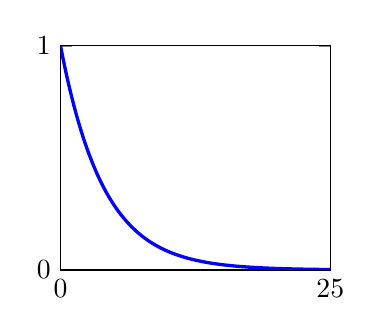
\begin{tikzpicture}
        \begin{axis}[
        domain = 0:25,
        scale=0.5,
        ytick = {0,1}, 
        xtick = {0,25},
        samples = 100,
        xmin=0, xmax=25,
        ymin=0, ymax=1,
        ]
        \addplot[color=blue, smooth, style = {very thick}]{exp(x*-0.25)};
        \end{axis}
        \end{tikzpicture}
    \end{center}
        
    \end{tcolorbox}
    \item Esperanza de vida o duración media de un disco.
    \begin{tcolorbox}[colback=white,colframe=cyan!50!black,fonttitle=\bfseries]
    Sabemos que: $E(t)= \int_0^{\infty}t*f(t)dt$\\
    Y que $f(t) = F'(t) = -R'(t)$\\
    
    Entonces: $f(t) = -(-\frac{1}{4}*e^{-t/4})= \frac{1}{4}e^{-t/4}$\\
    
    Y por tanto la esperanza de vida es: $E(t)= \int_0^{\infty}\frac{t}{4}e^{-t/4}dt = 4$
    \end{tcolorbox}
    \item El SCRUM Master ha estimado una duración de 3.5 años para el proyecto A y solicita el envío de un lote de 100 discos. ¿Cuál es el porcentaje de discos que aguantarán funcionando todo el proyecto?
    \begin{tcolorbox}[colback=white,colframe=cyan!50!black,fonttitle=\bfseries]
    Recordemos que $R(t)= P(T>t)$\\
    
    $P(T > 3.5) = R(3.5) = e^{-3.5/4}=0.4168 = 41.68\%$\\
    Entonces el $41.68\%$ de $100 = 41.68$
    \end{tcolorbox}
    \item Para prevenir problemas, el administrador de la red ha decidido comprar algunos discos más y tenerlos en reserva, pues el fabricante suele tardar unos 3 meses en realizar un nuevo envío. ¿Qué cantidad de discos extra debe comprar para asegurar que se pueda hacer el repuesto sin necesidad de esperar la entrega del fabricante?
    \begin{tcolorbox}[colback=white,colframe=cyan!50!black,fonttitle=\bfseries]
    $P(3meses>t)=P(\frac{1}{4}>t)=1-R(1/4)=F(1/4)=1-e^{-(0.25^2)}=0.0606=6.06\% \rightarrow 7$ discos.
    \end{tcolorbox}
    \item El proyecto B es un alojamiento de datos masivos de una red social. Para configurar el sistema el administrador necesita conocer lo siguiente: 
    \begin{itemize}
        \item ¿Qué duración $t_1$ no será superada por el 1\% de ellos?
        \item ¿Qué duración $t_1$ será superada por el 95\% de ellos?
    \end{itemize}
    \begin{tcolorbox}[colback=white,colframe=cyan!50!black,fonttitle=\bfseries]
    \begin{itemize}
        \item $P(T>t_0)\leq 0.99$; $R(t_0)\leq 0.99$; $e^{-t_0/4}\leq 0.99$; $-t_0/4 \leq ln(0.99)$; $-t_0 \leq 4*ln(0.99)$; $t_0 \geq 4*ln(0.99)$; $t_0 \geq 0.040$
        \item $P(T>t_1)\leq 0.95$; $R(t_1)\leq 0.95$; $e^{-t_1/4}\leq 0.95$; $-t_1/4 \leq ln(0.95)$; $-t_1 \leq 4*ln(0.95)$; $t_1 \geq 4*ln(0.95)$; $t_1 \geq 0.2051$
    \end{itemize}
    \end{tcolorbox}
\end{enumerate}

%%%%%%%%%%%%%%%%%%
\subsection{Ejercicio 2}
Un sistema informático posee una función de fiabilidad de
\[ R(t)=\begin{cases} 
      e^{-t} & 0<t<1 \\
      e^{-t^2} & 1\leq t 
   \end{cases}
\]
donde la duración está expresada en años. Se pide:
\begin{enumerate}
    \item Representar la fiabilidad y calcular la función de densidad de fallos.
    \begin{tcolorbox}[colback=white,colframe=cyan!50!black,fonttitle=\bfseries]
    La función de fiabilidad $R(t)$ se representa:
    \begin{center}
        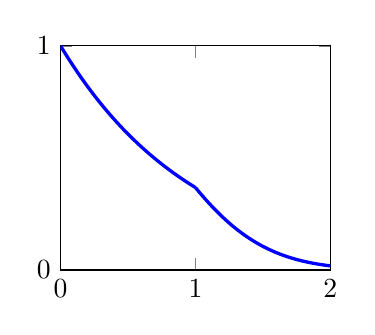
\begin{tikzpicture}
        \begin{axis}[
        scale=0.5,
        ytick = {0,1}, 
        xtick = {0,1,2},
        samples = 100,
        xmin=0, xmax=2,
        ymin=0, ymax=1,
        ]
        \addplot[color=blue, smooth, domain=0:1, style = {very thick}]{exp(-x)};
        \addplot[color=blue, smooth, domain=1:2, style = {very thick}]{exp(-x^2)};
        \end{axis}
        \end{tikzpicture}
    \end{center}
    Y la función de densidad de fallos es:
    \[ f(t)=-R'(t)=\begin{cases} 
      e^{-t} & 0<t<1 \\
      2t*e^{-t^2} & 1\leq t 
    \end{cases}
    \]
    \end{tcolorbox}
    \item La tasa de fallos. ¿Es constante en cualquier intervalo?
    \begin{tcolorbox}[colback=white,colframe=cyan!50!black,fonttitle=\bfseries]
    Recordemos que la tasa de fallos $\lambda(t) = \frac{f(t)}{R(t)}$, por tanto:
    \[ \lambda(t)=\begin{cases} 
      1 & 0<t<1 \\
      2t & 1\leq t 
    \end{cases}
    \]
    Es constante en el intervalo (0,1).
    \end{tcolorbox}
    \item Probabilidad de que el sistema falle durante el primer año.
    \begin{tcolorbox}[colback=white,colframe=cyan!50!black,fonttitle=\bfseries]
    $P(1<t)=1-R(1)=1-\frac{1}{e}= 0.6321$
    \end{tcolorbox}
    \item Probabilidad de que el sistema falle entre el segundo y el tercer año.
    \begin{tcolorbox}[colback=white,colframe=cyan!50!black,fonttitle=\bfseries]
    $P(2<t<3)=R(2)-R(3)=e^{-4}-e^{-9}= 0.01819$
    \end{tcolorbox}
\end{enumerate}

%%%%%%%%%%%%%%%%%%
\subsection{Ejercicio 3}
Sea T = tiempo hasta que se produce el primer intento de intrusión por determinados hackers en un sistema informático. Se conoce la función de riesgo
\[ \lambda(t)=\begin{cases} 
      0 & 0<t<1 \\
      \frac{2}{t} & t\geq 1 
   \end{cases}
\]
donde el tiempo se define en días. Se pide:
\begin{enumerate}
    \item Comprobar  que  se  trata  de  una  función  de  riesgo  real  calculando  y  analizando  la  fiabilidad  del modelo.
    \begin{tcolorbox}[colback=white,colframe=cyan!50!black,fonttitle=\bfseries]
    Sabemos que $R(t) = e^{-\int_0^t \lambda(s) ds}$.
    \begin{itemize}
        \item $0<t<1$ : $R(t)=e^{-\int_0^t 0 ds} = e^{-0}=1$
        \item $t\geq 1$ : $R(t)=e^{-\int_0^t \lambda(s) ds} = ... = 1/t^2$
    \end{itemize}
    \[ R(t)=\begin{cases} 
      1 & 0<t<1 \\
      \frac{1}{t^2} & t\geq 1 
   \end{cases}
    \]  
        \begin{center}
        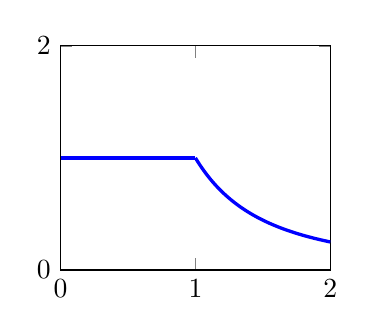
\begin{tikzpicture}
        \begin{axis}[
            scale=0.5,
            ytick = {0,2}, 
            xtick = {0,1,2},
            samples = 100,
            xmin=0, xmax=2,
            ymin=0, ymax=2,
        ]
        \addplot[color=blue, smooth, domain=0:1, style = {very thick}]{1};
        \addplot[color=blue, smooth, domain=1:2, style = {very thick}]{1/x^2)};
        \end{axis}
        \end{tikzpicture}
        \end{center}
        \end{tcolorbox}
    \item Calcular  el  tiempo  disponible  para  efectuar  una  transacción  electrónica  de  fundamental  seguridad para la empresa, desde que se pone en funcionamiento el SI.
    \begin{tcolorbox}[colback=white,colframe=cyan!50!black,fonttitle=\bfseries]
    Buscamos un $t_0$ : $P(T>t_0)=1$\\
    Queremos el máximo $t_0$ : $R(t_0)=1$, por tanto $t_0 = 1$
    \end{tcolorbox}
    \item Calcular la vida fiable de la variable asociada a un nivel de fiabilidad de 0.95 ¿Cada cuánto tiempo se recomienda cambiar la contraseña del sistema para garantizar dicha fiabilidad?
    \begin{tcolorbox}[colback=white,colframe=cyan!50!black,fonttitle=\bfseries]
    $P(T>t_1)\geq0.95$;\hspace{.5cm}$R(t_1)\geq0.95$;\hspace{.5cm}$\frac{1}{t^2_1}\geq0.95$;\hspace{.5cm}$t_1\leq 1.025$; 
    \end{tcolorbox}
\end{enumerate}

%%%%%%%%%%%%%%%%%%
\subsection{Ejercicio 4}
El  departamento  de  I+D  de  una  empresa,  ha  estimado  que  la  tasa  de fallos  de  un  procesador  de  última generación es
\[ \lambda(t)=\begin{cases} 
      \frac{1}{1+t} & 0<t<1 \\
      0.5 & t\geq 1
   \end{cases}
\]
Sabiendo que el tiempo se mide en cientos de miles de horas, se pide:
\begin{enumerate}
    \item Calcular la función de distribución y la función de fiabilidad.
    \begin{tcolorbox}[colback=white,colframe=cyan!50!black,fonttitle=\bfseries]
    Primero calculamos la función de fiabilidad $R(t) = e^{-\int_0^t \lambda(s) ds}$.
    \begin{itemize}
        \item Si $0<t<1$: $R(t)=e^{-\int_0^t \frac{1}{1+s} ds} = e^{-ln(1+t)} = \frac{1}{1+t}$
        \item Si $t \geq 1$: $R(t)=\frac{1}{2}e^{\frac{1-t}{2}}$
    \end{itemize}
    Por tanto:
    \[ R(t)=\begin{cases} 
      \frac{1}{1+t} & 0<t<1 \\
      \frac{1}{2}e^{\frac{1-t}{2}} & t\geq 1
   \end{cases}
    \]
    Y sabiendo que $F(t) = 1-R(t)$, calculamos la función de distribución:
    \[ F(t)=\begin{cases} 
      1-\frac{1}{1+t} & 0<t<1 \\
      1-(\frac{1}{2}e^{\frac{1-t}{2}}) & t\geq 1
   \end{cases}
    \]
    \end{tcolorbox}
    \item Calcular la vida media de dichos procesadores.
    \begin{tcolorbox}[colback=white,colframe=cyan!50!black,fonttitle=\bfseries]
    La vida media se define como: $E(t)= \int_0^{\infty}t*f(t)dt$\\
    Por lo que primero necesitamos conocer la densidad de fallos $f(t)$.
    \[
    f(t)=-R'(t)=\begin{cases} 
      \frac{1}{(1+t)^2} & 0<t<1 \\
      \frac{1}{4}e^{\frac{1-t}{2}} & t\geq 1
   \end{cases}
    \]
    Y ahora calculamos $E(t)$
    \[
    E(t)= \int_0^{\infty}t*f(t)dt= \int_0^1\frac{t}{(1+t)^2}dt + \int_1^{\infty}\frac{t}{4}e^{\frac{1-t}{2}}dt = 1.643
    \]
    \end{tcolorbox}
\end{enumerate}
%%%%%%%%%%%%%%%%%%
\subsection{Ejercicio 5}
Para diseñar un sistema de comunicaciones se dispone de 10 componentes idénticos e independientes. El administrador quiere calcular la esperanza de vida de distintos diseños:
\begin{enumerate}
    \item Diseño en serie de 10: Suponiendo que las componentes tienen distribución exponencial y una duración media de cada componente de 8000 horas, que es lo que se ha estimado a partir de una muestra anterior.
    \begin{tcolorbox}[colback=white,colframe=cyan!50!black,fonttitle=\bfseries]
    Si la esperanza de vida media de 1 componente son 8000 horas, la esperanza de vida de 10 componentes en serie será $E(S_{10})=\frac{8000}{10}=800$ horas.
    \end{tcolorbox}
    \item Diseño en serie de 10 tras un estudio más minucioso que revela que la duración  de los componentes sigue realmente una distribución de Weibull con $k=2$ y $\lambda=10$.
    \begin{tcolorbox}[colback=white,colframe=cyan!50!black,fonttitle=\bfseries]

    \end{tcolorbox}
    \item Diseño en paralelo de dos series de 5 con la distribución anterior. En  este  caso, en lugar de la esperanza de vida se pide:
    \begin{enumerate}
        \item Calcular la probabilidad de que el sistema siga funcionando al cabo de 500 horas.
        \item Calcular la probabilidad de que el sistema siga funcionando al cabo de 5000 horas.
    \end{enumerate}
    \begin{tcolorbox}[colback=white,colframe=cyan!50!black,fonttitle=\bfseries]

    \end{tcolorbox}
\end{enumerate}
%%%%%%%%%%%%%%%%%%
\subsection{Ejercicio 6}
El  proceso  de  arranque  de  cierto  tipo  de  procesadores  invadido  por un  virus  informático  presenta  una duración hasta fallo (en minutos)modelizada mediante la siguiente distribución:
\[ F(t)=\begin{cases} 
      \frac{1}{10}(t^3+t) & 0<t<2 \\
      1 & t\geq 2 
   \end{cases}
\]
Sabiendo que el sistema de arranque normal tarda 180 segundos, se pide:
\begin{enumerate}
    \item Hallar la función de fiabilidad del proceso de arranque y la función de riesgo asociada.
    \begin{tcolorbox}[colback=white,colframe=cyan!50!black,fonttitle=\bfseries]

    \end{tcolorbox}\textbf{}
    \item Calcular el porcentaje de procesadores que completará el proceso de arranque con éxito.
    \begin{tcolorbox}[colback=white,colframe=cyan!50!black,fonttitle=\bfseries]

    \end{tcolorbox}
    \item Para  resolver  el  problema,  la  organización  ha  decidido instalar  un  antivirus  que  tarda  1  minuto  en eliminar  el  virus atacante.  Si  la  organización  posee  2000  equipos,  ¿cuántos  de  ellos se  espera  que realicen bien el proceso de arranque?
    \begin{tcolorbox}[colback=white,colframe=cyan!50!black,fonttitle=\bfseries]

    \end{tcolorbox}
\end{enumerate}